\section{Die Untersuchung der Genauigkeit der Selektoren}
\label{sec:evaluierung}

In diesem Kapitel wird untersucht, wie gut der Extraktionsalgorithmus funktioniert.
Dazu wird zunächst die Qualität der idealo-Daten, welche zum Anlernen und zum Evaluieren genutzt wird, grob analysiert.
Mit Hilfe der durchgeführten Messungen werden abschließend die Auswirkungen der Ergebnisse auf das Matching abgeleitet.

\subsection{Die Testdaten}
\label{subsec:testdaten}

Sowohl für das Antrainieren der Regeln als auch für das Evaluieren des Parsers werden Daten von idealo genutzt.
Für die nachfolgenden Messungen wurden Angebote von 50 Shops verwendet.
Für jeden Shop wurden 150 Angebote geladen.
Maximal 50 der 150 Angebote werden für das Anlernen verwendet.
Die Evaluation findet mit den restlichen 100 Angeboten statt.

Nachfolgend soll ein grober, quantitativer Überblick über die idealo-Daten gegeben werden.

\begin{figure}[H]
    \centering
    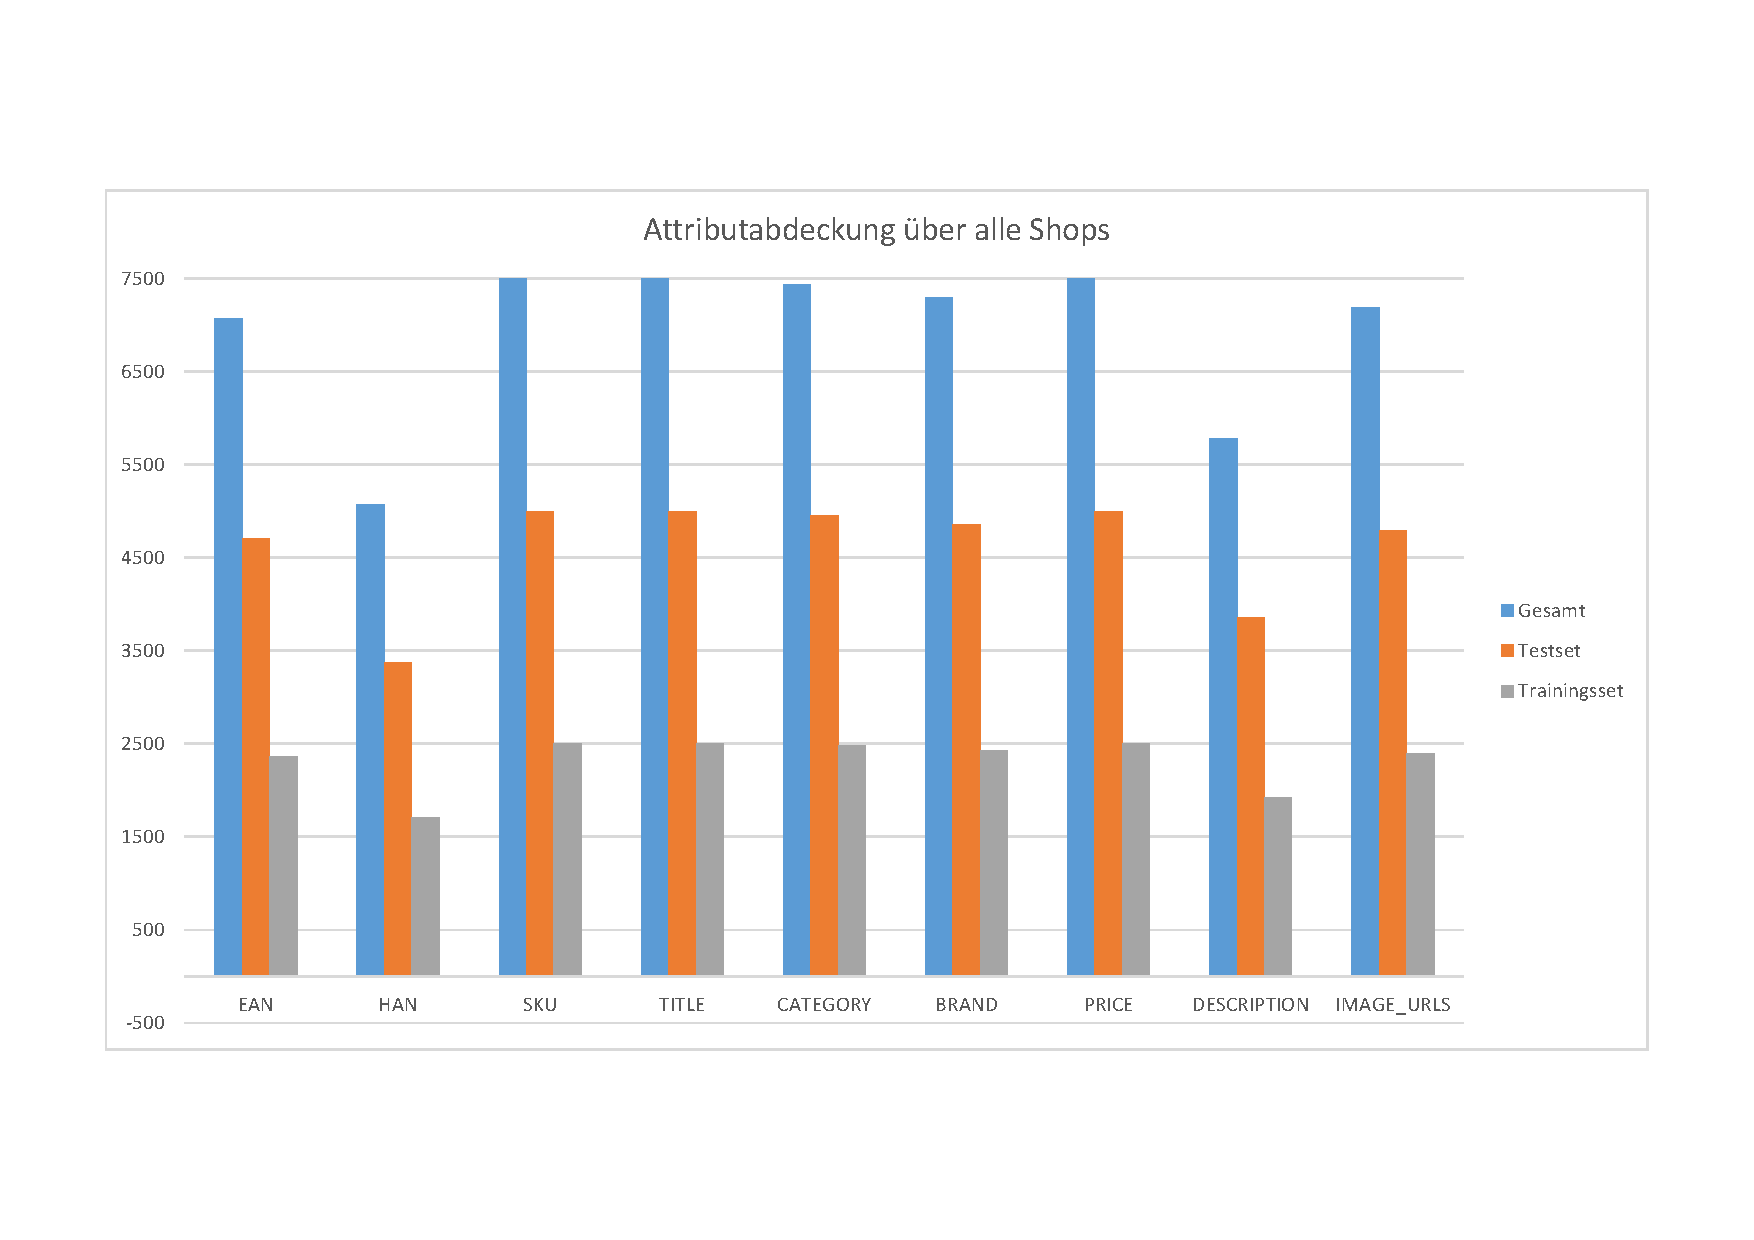
\includegraphics[width=\textwidth, trim=1.5cm 9.5cm 1.5cm 11cm, clip]{resources/Attributabdeckung-idealo-Daten.pdf}
    \caption{Attributabdeckung der idealo-Daten}
    \label{abb:testdaten}
\end{figure}

Der Abbildung~\ref{abb:testdaten} kann man entnehmen, dass es für jedes untersuchte Angebot einen Titel, einen Preis
und die SKU gibt.
Interessanterweise sind andere Produkteigenschaften, welche für die eindeutige Zuordnung genutzt werden können,
häufiger nicht vorhanden.
Der Verlauf der Attributabdeckung ähnelt sich in allen Datenreihen.
Die Verteilungen der Attribute innerhalb des Test- und des Trainingsset sind also ähnlich.